%%%%%%%%%%%%%%%%%%%%%%%%%%%%%%%%%%%%%%%%%
% Lachaise Assignment
% LaTeX Template
% Version 1.0 (26/6/2018)
%
% This template originates from:
% http://www.LaTeXTemplates.com
%
% Authors:
% Marion Lachaise & François Févotte
% Vel (vel@LaTeXTemplates.com)
%
% License:
% CC BY-NC-SA 3.0 (http://creativecommons.org/licenses/by-nc-sa/3.0/)
% 
%%%%%%%%%%%%%%%%%%%%%%%%%%%%%%%%%%%%%%%%%

%----------------------------------------------------------------------------------------
%	PACKAGES AND OTHER DOCUMENT CONFIGURATIONS
%----------------------------------------------------------------------------------------

\documentclass{article}
\usepackage{amsthm}
\usepackage{listings}
\usepackage{xcolor}
\usepackage{graphicx}


\lstset{
	language=Python,
	basicstyle=\ttfamily\small,
	keywordstyle=\color{blue},
	stringstyle=\color{red},
	commentstyle=\color{purple},
	showstringspaces=false,
	numbers=left,
	numberstyle=\tiny\color{gray},
	breaklines=true,
	frame=single,
	captionpos=b
}
\newtheorem{definition}{Definition}[section]
\newtheorem{proposition}{Proposition}
\newtheorem{corolary}{Corolary}

\input{structure.tex} % Include the file specifying the document structure and custom commands

%----------------------------------------------------------------------------------------
%	ASSIGNMENT INFORMATION
%----------------------------------------------------------------------------------------

\title{LISTA 2 DE MAC5770 - ÁRVORES E GRAFOS EULERIANOS} % Title of the assignment

\author{Giovani Tavares (10788620)\\ \texttt{giovanitavares@usp.br}} % Author name and email address

\date{University of Sao Paulo --- 2025.1} % University, school and/or department name(s) and a date

%----------------------------------------------------------------------------------------

\begin{document}

\maketitle % Print the title

%----------------------------------------------------------------------------------------
%	INTRODUCTION
%----------------------------------------------------------------------------------------

\section{12 de Maio, 2025} % Unnumbered section


 \subsection{Exercício 1:  Seja $G$ um grafo simples de ordem $n$, $n$ par. Prove que se $d(v) > n/2$ para todo $v \in V (G)$, então $G$ contém $3$ emparelhamentos perfeitos dois a dois disjuntos.}
 
 \section*{Parte I}
 
 Mostrando que todo ciclo hamiltoniano pode ser escrito como a união de dois emparelhamentos perfeitos disjuntos.
 
 Pelo Teorema de Dirac, se $d(v) > n/2$, então $G$ tem um ciclo hamiltoniano.
 
 Seja $H = (v_1, v_2, \ldots, v_n, v_1)$, um ciclo hamiltoniano de $G$.
 
 Podemos escrever o ciclo $H$ como um conjunto de arestas:
 
 $$
 H = \{ \{v_1, v_2\}, \{v_2, v_3\}, \ldots, \{v_{n-1}, v_n\}, \{v_n, v_1\} \}
 $$
 
 Ou seja, podemos escrever $H$ como a união de dois conjuntos disjuntos de arestas:
 
 $$
 H = \left[ \{ \{v_1, v_2\}, \{v_3, v_4\}, \{v_5, v_6\}, \ldots, \{v_{n-1}, v_n\} \} \right] \cup
 \left[ \{ \{v_2, v_3\}, \{v_4, v_5\}, \{v_6, v_7\}, \ldots, \{v_n, v_1\} \} \right]
 $$
 
 Ou seja, podemos escrever $H$ como a união de dois conjuntos disjuntos de arestas:
 
 $$
 A = \bigcup_{i \text{ ímpar}}^{n-1} \{ \{v_i, v_{i+1}\} \}, \quad 
 B = [\bigcup_{j \text{ par}}^{n-1} \{ \{v_j, v_{j+1}\} \}] \cup \{ \{v_n, v_1\} \}
 $$
 
 $A$ é emparelhamento perfeito, pois cobre os $n$ vértices de $G$ e não contém arestas adjacentes, o mesmo valendo para $B$. Além disso, $A$ e $B$ são disjuntos, pois uma aresta $\{v_i, v_{i+1}\}$ não pode ter $i$ par e ímpar simultaneamente (i.e., não pode estar em $A$ e $B$ ao mesmo tempo).
 
 Assim, o ciclo hamiltoniano $H$ pode ser escrito como a união de dois emparelhamentos perfeitos disjuntos. Como $H$ é arbitrário, pode-se concluir que todo ciclo hamiltoniano pode ser escrito como a união de dois emparelhamentos perfeitos disjuntos.
 
 \section*{Parte II}
 
 Mostrando que, se $G$ é tal que $v(G) = n$, $n$ par, e $d(v) > n/2$ para todo vértice $v$ de $G$, então $G$ tem 3 emparelhamentos perfeitos dois a dois disjuntos.
 
 Como $\forall v \in V(G)$, $d(v) > n/2$, então, pelo Teorema de Dirac, $G$ tem um ciclo hamiltoniano $H$. 
 
 Como demonstrado anteriormente na \textbf{Parte I}, $H$ pode ser escrito como a união de dois emparelhamentos perfeitos. Chamemos-nos de $M_1$ e $M_2$:
 
 $$
 H = M_1 \cup M_2
 $$
 
 Pode-se afirmar que $G$ tem 2 emparelhamentos perfeitos disjuntos.
 
 Seja $G' = G \setminus M_1$, o grafo formado pela retirada das arestas de $M_1$ de $G$.
 
 Como $M_1$ é emparelhamento perfeito, temos que $\forall v \in V(G), d_{M_1} = 1$, entao: 
 
 Portanto:
 
 $$
 d_{G'}(v) = d_G(v) - d_{M_1}  =  d_G(v) - 1
 $$
 
 Com $d_G(v) > n/2$ e $n$ par. Como $d_G(v) \in \mathbb{Z}$, temos:
 
 \begin{align*}
 	d_G(v) &> \frac{n}{2} \\
 	\implies d_{G}(v) &\geq \frac{n}{2}  + 1\\
    \implies d_G(v) - 1 &\geq (\frac{n}{2} + 1) - 1 \\
  	\implies d_{G'}(v) &\geq \frac{n}{2}
 \end{align*}
 
 Assim, pelo Teorema de Dirac, $G'$ também tem um ciclo hamiltoniano $H'$. Como demonstrado na \textbf{Parte I}, $H'$ pode ser escrito como a união de dois emparelhamentos perfeitos disjuntos $M_3$ e $M_4$:
 
 $$
 H' = M_3 \cup M_4
 $$
 
 Sabemos que $M_3$ e $M_4$ também são emparelhamentos perfeitos de $G$, pois $V(G) = V(G')$ e $E(G') \subset E(G)$.
 
 Além disso, $M_1 \cap M_3 = M_1 \cap M_4 = \varnothing$, pois as arestas de $M_1$ foram removidas para formar $G'$. 
 
 Assim, $M_1, M_3$ e $M_4$ são três emparelhamentos perfeitos dois a dois disjuntos de $G$ e, portanto, $G$ tem $3$ emparelhamentos perfeitos dois a dois disjuntos.
 
 \clearpage
 
 \subsection{Exercício 2:  Prove que toda árvore tem no máximo um emparelhamento perfeito. De um exemplo de uma árvore sem emparelhamento perfeito.}

Utilizemos uma prova por inducao.


  \subsubsection*{Caso Base}
  
  Seja $T$ uma árvore com dois vértices. O emparelhamento perfeito de $T$ contém a única aresta de $T$ e é único, pois nao existe apenas uma aresta incidente a seus dois únicos vértices.
  
  
  
  \subsubsection*{Hipótese de Inducao}
  
  Suponhamos que toda árvore $T$ com $k < n$ vértices seja tal que tenha no máximo um emparelhamento perfeito.
  
  Seja $T$ uma árvore com $n$ vértices, i.e., $v(T) = n$. Seja $M$ um emparelhamento perfeito de $T$.

 $T$ é árvore, entao $V(T)$ tem pelo menos um vértice $f$ que é folha, i.e., um vértice $f$ tal que $d_T(f) = 1$.
  
Como $d_T(f) = 1$, existe um vértice $u \neq f$, $u \in V(T)$, tal que $u$ é vizinho de $f$.
  
Seja $F$ a floresta formada pela retirada dos vértices $u$ e $f$ de $T$, i.e., 

\begin{align*}
	E(F) &=  E(T) \setminus  \{   \{u,f\}   \} \\
	V(F) &=  V(T) \setminus \{u,f\} \\
	&\implies v(F) = v(T) - 2 = n - 2 < n \\
	&\implies \text{F tem no máximo um emparelhamento perfeito, pela hipótese de inducao.}  \\
\end{align*}

Chamemos $M'$ o emparelhamento perfeito único de $F$. Como $F$ tem exatamente as mesmas arestas de $T$ com exececao da única incidente a $f$, chamada $\{u,f\}$, pode-se afirmar que a adicao da aresta $\{\{u,f\}\}$ a $M'$ recupera $M$, i.e. :

\begin{align}
	M = M' \cup \{\{u,f\}\}
\end{align}

Como $\{u,f\}$ é a única aresta incidente a $f$ na árvore $T$, pois $f$ é folha, $\{u,f\}$ é aresta presente em qualquer emparelhamento perfeito de $T$. Assim, para gerar emparelhamento perfeito de $T$ distinto de $M$, é preciso substituir pelo menos uma aresta $e'$ de $M'$ por alguma aresta $e_{sub} \in E(T)$ nao presente entre as arestas de $M'$, formando o conjunto de arestas $M''$.  $e_{sub} \neq \{u,v\}$, pois $e_{sub}$ deve ser incidente a pelo menos um dos vértices aos quais incide $e'$, e os vértices $u$ e $f$ nao estao entre os vértices das arestas de $M'$.

 $M'$ é emparelhamento perfeito único da floresta $F$ por hipótese, o que indica que nao existe nenhum outro conjunto de arestas nao adjascentes que cubram todos os vértices de $F$, i.e., $M''$ nao é emparelhamento. Assim, 


\begin{align}
	M = M'' \cup \{\{u,f\}\}
\end{align}

é uma contradicao, pois $M$ nao pode ser um emparelhamento perfeito com um subconjunto de arestas $M''$ que nao é um emparelhamento. 

Assim, o emparelhamento $M$ é único e tal que

\begin{align}
	M = M' \cup \{\{u,f\}\}
\end{align}

Estando demonstrado que vale a afirmacao vale para árvores $T$ tais que $v(T) = n$


 \subsubsection*{Exemplo de árvore sem emparelhamento perfeito}

 A árvore definida por 
 
 \begin{align*}
 	E(T) &=  \{\{u_1,u_2\},\{u_2,u_3\}    \} \\
 	V(T) &=  \{u_1,u_2,u_3\}
 \end{align*}
 
  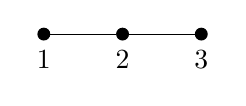
\begin{tikzpicture}
 	% Define the vertices
 	\node[circle, draw, fill=black, inner sep=1.5pt, label=below:1] (v1) at (0,0) {};
 	\node[circle, draw, fill=black, inner sep=1.5pt, label=below:2] (v2) at (1,0) {};
 	\node[circle, draw, fill=black, inner sep=1.5pt, label=below:3] (v3) at (2,0) {};
 	
 	% Draw the edges
 	\draw (v1) -- (v2);
 	\draw (v2) -- (v3);
 \end{tikzpicture}
 
 Nao tem emparelhamento perfeito, pois tem um número ímpar de vértices.
\clearpage


 \subsection{Exercício 3:  Seja $G$ um grafo $(X, Y)-\text{bipartido}$ simples tal que $|X| = |Y | = n \geq 1$. Prove que se $e(G) > n(n - 1)$ então $G$ tem um emparelhamento perfeito.}
 
 Suponhamos, por absurdo, que $G$ não tem um emparelhamento perfeito. Então, pelo Teorema de Hall, $\exists S \subseteq X$ tal que $|N(S)| < |S|$. Seja $|S| = s$.
 
 O objetivo é chegar em uma contradição e encontrar um limite superior para $e(G)$ sob a suposição. Pode-se afirmar:
 
 $$1 \leq s \leq n - 1,$$ pois $s = |S|$ e $S \subset X$.  
 $$|N(S)| < s$$ por suposição.
 
 Cada vértice de $S$ está conectado a somente vértices em $N(S)$. Assim, o número máximo de arestas entre $S$ e $N(S)$ é igual ao produto de $s$ com $|N(S)|$, i.e.,
 
 $$\sum_{u \in S} d(u) \leq |S| \cdot |N(S)| = s \cdot |N(S)|$$  
 que corresponde ao número máximo de arestas adjascentes aos vértices de $S$, pois $S \subseteq X$ e $G$ é $(X, Y)-\text{bipartido}$.
 
 Cada vértice de $X \setminus S$ pode estar conectado a qualquer vértice de $Y$, exceto aos vértices de $Y$ conectados a $S$ (i.e., exceto aos vértices de $N(S)$).
 
 Assim, o número máximo de arestas de $X \setminus S$ para $Y$ é:
 
 $$\sum_{v \in X \setminus S} d(v) \leq |X \setminus S| \cdot |Y| = (n - s) \cdot n$$
 
 Todas as arestas de $G$ são incidentes a algum vértice de $S$ ou de $X \setminus S$. Assim:
 
 
 \begin{align*}
 	\sum_{u \in S} d(u) + \sum_{v \in X \setminus S} d(v) &= e(G) \\
 	\implies s \cdot |N(S)| + n \cdot (n - s) &> n \cdot (n - 1), \quad \text{pois } e(G) > n \cdot (n - 1) \\ 
 	\implies s \cdot |N(S)| + n \cdot (n - s) &> n \cdot (n - 1) \\
 \end{align*}
 
 Como  $s \leq n - 1$ e  $|N(S)| < s$ por suposicao, temos que $|N(s)| \leq n - 2$. Assim:
 
  \begin{align*}
 	s \cdot |N(S)| + n \cdot (n - s) &> n \cdot (n - 1) \\
 	\implies (n-1)\cdot (n-2) + n \cdot (n - (n-1)) &> n \cdot (n - 1) \\
 	 \implies (n-1)\cdot (n-2) + n &> n \cdot (n - 1) \\
 	\implies (n-1)\cdot (n-2) &> n^2 - n - n \\
 	 \implies (n-1)\cdot (n-2) &> n \cdot (n - 2), \quad \text{o que é um absurdo, pois} \quad n \geq 1\\
 \end{align*}
 
Assim, a suposicao inicial está incorreta e, portanto, $\forall S \subset X, |N(S)| \geq |S|$. 

Pelo Teorema de Hall, existe um emparelhamento que cobre $X$. Como $(X, Y)$ é uma bipartição de $G$, qualquer emparelhamento $M$ que cubra $X$ deve ser formado exclusivamente por arestas incidentes a um vértice de $X$ e a outro vértice de $Y$.

Além disso, $M$ é emparelhamento perfeito de $X$, entao $M$ nao possui pares de arestas adjascentes, i.e., cada vértice de $X$ coberto por $M$ está exclusivamente ligado a um vértice de $Y$. Como $|X| = n$, há $n$ vértices distintos de $Y$ ligados aqueles de $X$ em $M$. Como $|Y| = n$, conclui-se que $M$ também cobre $Y$. Portanto, $M$ é emparelhamento perfeito de $G$.

\clearpage





\end{document}
